% The model, drawn from the code (results/research/retouch_unified_20260929/train_ru_clip.py RUCLIP, train_ru5.py RUCLIP5 and
% loss_fn, train_ru3.py footprint / mask_loss) and the checkpoint ru_clipe5_s20260929.pth (96 LoRA adapters A 16x1024,
% B 1024x16; heads fz 2x1024, pres 4x1024, q 4x1024, ev 1x1024; 3,157,003 trained parameters; frozen CLIP vision tower
% 303,179,776). Tiles: make_tiles_model.py (held-out FF++ test frame 682, nose from a donor). Build: make_fig_model.sh.
% Row 1: the image encoder with one Transformer block and its LoRA adapter enlarged. Row 2: the heads.
\documentclass[border=0pt]{standalone}
\usepackage{fontspec}
\setmainfont{Liberation Sans}
\usepackage{tikz}
\usetikzlibrary{arrows.meta,positioning,calc,shapes.geometric,fit,backgrounds}
\definecolor{nn}{HTML}{0F4D92}
\definecolor{code}{HTML}{1B7F4C}
\definecolor{ink}{HTML}{222222}
\definecolor{muted}{HTML}{5E6670}
\definecolor{frz}{HTML}{8C939B}
\definecolor{fk}{HTML}{D55E00}
\definecolor{rl}{HTML}{009E73}
\definecolor{bt}{HTML}{B07800}
\definecolor{fp}{HTML}{26A6DC}
\definecolor{panel}{HTML}{F4F6F9}
\definecolor{pline}{HTML}{C9D1DB}
\newcommand{\vi}[1]{\textit{#1}}
\newcommand{\sg}[1]{σ\textsubscript{\textit{#1}}}
\begin{document}
\fontsize{9}{10.8}\selectfont
\hyphenpenalty=10000 \exhyphenpenalty=10000
\begin{tikzpicture}[
  x=1cm, y=1cm, text=ink,
  >={Latex[length=1.7mm,width=1.5mm]},
  ar/.style={->, line width=0.6pt, draw=ink},
  ln/.style={line width=0.6pt, draw=ink},
  fr/.style={draw=frz, fill=frz!14, rounded corners=1.5pt, line width=0.5pt, align=center, inner sep=1.5pt},
  tr/.style={draw=nn, fill=nn!9, rounded corners=1.5pt, line width=0.9pt, align=center, inner sep=1.5pt},
  lab/.style={align=center, inner sep=0pt},
  tok/.style={draw=frz, fill=frz!22, minimum width=0.66cm, minimum height=0.30cm, inner sep=0pt, line width=0.4pt},
  pl/.style={circle, draw=ink, line width=0.6pt, minimum size=0.30cm, inner sep=0pt, path picture={
      \draw[line width=0.6pt] ([xshift=-0.09cm]path picture bounding box.center) -- ([xshift=0.09cm]path picture bounding box.center);
      \draw[line width=0.6pt] ([yshift=-0.09cm]path picture bounding box.center) -- ([yshift=0.09cm]path picture bounding box.center);}},
]
% ================================================================ row 1: image encoder
% ---- input, patch embedding, tokens
\node[inner sep=0pt, anchor=south west] (in) at (0,7.05) {
\includegraphics[width=1.4cm]{figs/model_in.png}};
\foreach \i in {1,...,15} {
  \draw[white, opacity=0.6, line width=0.2pt] ($(in.south west)+(\i*1.4/16,0)$) -- ++(0,1.4);
  \draw[white, opacity=0.6, line width=0.2pt] ($(in.south west)+(0,\i*1.4/16)$) -- ++(1.4,0);
}
\node[lab, anchor=south west, align=left] at (0,8.55) {\textbf{input}\\224×224 crop,\\16×16 patches};

\node[tok, fill=frz!50, anchor=south west] (t0) at (3.04,8.5) {CLS};
\foreach \k in {1,...,4} { \node[tok, below=0.04cm of t\the\numexpr\k-1\relax] (t\k) {}; }
\node[lab, below=0cm of t4] (tdots) {$\vdots$};
\node[tok, below=0cm of tdots] (t5) {};
\draw[ar] (in.east |- t2.west) -- node[below=2pt, lab] {patch\\embedding\\588→1024} (t2.west);

% ---- encoder box
\node[draw=pline, fill=panel, rounded corners=6pt, line width=0.6pt, minimum width=9.0cm, minimum height=6.0cm,
      anchor=south west] (enc) at (3.75,4.75) {};
\node[fill=nn, text=white, font=\fontsize{10}{12}\selectfont\bfseries, rounded corners=6pt, inner xsep=7pt, inner ysep=3pt,
      anchor=west] at ($(enc.north west)+(0.15,0)$) {CLIP ViT-L/14 image encoder \textmd{(frozen, 303.2 M)}};

% ---- one Transformer block, bottom to top
\def\bx{5.35}
\node[fr, minimum width=2.3cm, minimum height=0.40cm] (ln1) at (\bx,5.75) {LayerNorm};
\node[tr, minimum width=2.3cm, minimum height=0.95cm] (att) at (\bx,6.85) {multi-head\\attention\\16 heads};
\node[pl] (p1) at (\bx,7.8) {};
\node[fr, minimum width=2.3cm, minimum height=0.40cm] (ln2) at (\bx,8.35) {LayerNorm};
\node[fr, minimum width=2.3cm, minimum height=0.70cm] (mlp) at (\bx,9.1) {MLP\\1024→4096→1024};
\node[pl] (p2) at (\bx,9.85) {};
\draw[ln] (t5.south) |- (\bx,5.0);
\draw[ar] (\bx,5.0) -- (ln1.south);
\draw[ar] (ln1.north) -- (att.south);
\draw[ar] (att.north) -- (p1.south);
\draw[ar] (p1.north) -- (ln2.south);
\draw[ar] (ln2.north) -- (mlp.south);
\draw[ar] (mlp.north) -- (p2.south);
\draw[ar] (\bx,5.25) -| (3.98,7.8) -- (p1.west);
\draw[ar] (\bx,8.03) -| (3.98,9.85) -- (p2.west);
\node[draw=frz, dashed, rounded corners=3pt, line width=0.5pt, fit={(3.86,5.12) (7.08,10.08)}, inner sep=0pt] (blk) {};
\node[lab, anchor=east, font=\fontsize{11}{12}\selectfont\bfseries] at (7.0,6.85) {×24};

% ---- LoRA, enlarged from the attention block
\draw[nn, dashed, line width=0.4pt] (att.north east) -- (7.3,9.6);
\draw[nn, dashed, line width=0.4pt] (att.south east) -- (7.3,5.05);
\draw[nn, dashed, rounded corners=3pt, line width=0.4pt, fill=white] (7.3,5.05) rectangle (12.6,9.6);
\def\lx{9.0}
\node[fr, minimum width=1.5cm, minimum height=1.45cm] (w0) at (8.25,7.0) {\vi{W}\textsuperscript{0}\\1024×1024\\frozen};
\node[trapezium, trapezium angle=60, draw=nn, fill=nn!9, line width=0.9pt, minimum width=1.15cm, minimum height=0.5cm,
      inner sep=0pt, shape border rotate=180] (A) at (9.85,6.45) {\vi{A}};
\node[trapezium, trapezium angle=60, draw=nn, fill=nn!9, line width=0.9pt, minimum width=1.15cm, minimum height=0.5cm,
      inner sep=0pt] (B) at (9.85,7.6) {\vi{B}};
\node[pl] (p3) at (\lx,8.55) {};
\draw[ln] (\lx,5.45) -- (\lx,5.8);
\draw[ar] (\lx,5.8) -| (w0.south);
\draw[ar] (\lx,5.8) -| (A.south);
\draw[ar] (A.north) -- (B.south);
\draw[ar] (w0.north) |- (p3.west);
\draw[ar] (B.north) |- (p3.east);
\draw[ar] (p3.north) -- (\lx,8.92);
\node[lab, anchor=north] at (\lx,5.43) {\vi{x}};
\node[lab, anchor=south] at (\lx,8.95) {\vi{h} = \vi{W}\textsuperscript{0}\vi{x} + 2\,\vi{BAx}};
\node[lab, anchor=north west, align=left, text width=1.95cm] at (10.62,9.45)
  {\textbf{LoRA} on \vi{W}\textsubscript{q}, \vi{W}\textsubscript{k}, \vi{W}\textsubscript{v}, \vi{W}\textsubscript{o}
   of all 24 blocks: 96 adapters.\\[3pt]
   rank \vi{r} = 16:\\\vi{A}: 16×1024\\\vi{B}: 1024×16, starts at 0\\[3pt]
   \textcolor{nn}{3.15 M trained}};

% ---- output tokens
\node[tok, fill=frz!50, anchor=south west] (u0) at (13.0,8.5) {CLS};
\foreach \k in {1,...,4} { \node[tok, below=0.04cm of u\the\numexpr\k-1\relax] (u\k) {}; }
\node[lab, below=0cm of u4] (udots) {$\vdots$};
\node[tok, below=0cm of udots] (u5) {};
\draw[ar] (p2.east) -| (u0.north);

% ---- legend (left, below the input)
\node[fr, minimum width=0.42cm, minimum height=0.26cm, anchor=west] (lg1) at (0,6.2) {};
\node[lab, anchor=west] at ($(lg1.east)+(0.1,0)$) {frozen};
\node[tr, minimum width=0.42cm, minimum height=0.26cm, anchor=west] (lg2) at (0,5.75) {};
\node[lab, anchor=west] at ($(lg2.east)+(0.1,0)$) {trained};
\node[lab, anchor=north west, align=left] at (0,5.4) {3.16 M trained\\of 306 M};

% ================================================================ row 2: heads
% routes: patch tokens down and left to the evidence head; CLS right and down to the bus of the three heads
\draw[ln] (u5.south) -- (13.33,4.5) -- (1.1,4.5);
\draw[ln] (u0.east) -- (14.3,8.65) -- (14.3,4.05) -- (8.85,4.05);

% ---- evidence head on the 256 patch tokens
\node[tr, minimum width=2.2cm, minimum height=0.65cm] (he) at (1.1,3.0) {evidence head\\linear, per token};
\draw[ar] (1.1,4.5) -- (he.north);
\node[lab, anchor=north west, muted] at (1.25,4.42) {256 patch tokens};
\node[inner sep=0pt, anchor=west] (ev) at (2.6,2.75) {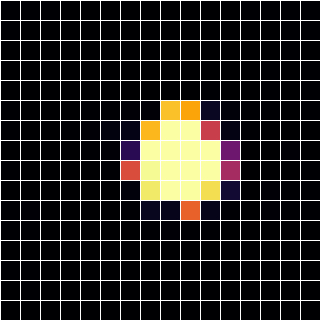
\includegraphics[width=1.6cm]{figs/model_ev16.png}};
\node[inner sep=0pt, anchor=west] (M) at (4.85,2.75) {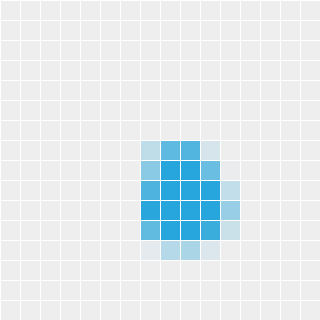
\includegraphics[width=1.6cm]{figs/model_M16.png}};
\draw[ar] (he.east) -- (ev.west);
\node[lab, anchor=south] at ($(ev.north)+(0,0.05)$) {map \vi{m}, 16×16};
\node[lab, anchor=south] at ($(M.north)+(0,0.05)$) {footprint \vi{M}};
\draw[<->, line width=0.8pt, draw=fp] (ev.east) -- (M.west);
\node[lab, anchor=north] at ($(ev.south)!0.5!(M.south)+(0,-0.08)$) {training: BCE + Dice};
\node[lab, anchor=north west, align=left, text=code] at (0,1.25)
  {page: MediaPipe landmarks → part masks → named part\\\textbf{nose} (mean evidence 0.99 on this held-out forgery)};

% ---- three heads on the pooled CLS token
\node[tr, minimum width=2.9cm, minimum height=0.65cm] (hz) at (8.85,3.4) {forged \vi{f}, beautified \vi{b}\\1024→2};
\node[tr, minimum width=1.9cm, minimum height=0.65cm] (hp) at (11.4,3.4) {operations\\1024→4};
\node[tr, minimum width=1.9cm, minimum height=0.65cm, draw=nn!45, fill=nn!3] (hq) at (13.5,3.4) {quantities\\1024→4};
\draw[ar] (8.85,4.05) -- (hz.north);
\draw[ar] (11.4,4.05) -- (hp.north);
\draw[ar] (13.5,4.05) -- (hq.north);
\node[lab, anchor=east, muted] at (8.7,4.05) {pooled CLS token};
\node[lab, anchor=north, align=left] at ($(hz.south)+(0,-0.15)$)
  {\textcolor{fk}{forged = \sg{f}}\\[1pt]\textcolor{bt}{beautified = (1−\sg{f})\,\sg{b}}\\[1pt]\textcolor{rl}{real = (1−\sg{f})(1−\sg{b})}};
\node[lab, anchor=north, align=center] at ($(hp.south)+(0,-0.15)$) {σ: eye, contour,\\tone, texture};
\node[lab, anchor=north, align=center, muted] at ($(hq.south)+(0,-0.15)$) {4 measured\\amounts,\\auxiliary};

% ================================================================ side card: training (full text width 18.13 cm)
\node[anchor=north west, align=left, text width=2.8cm, inner sep=0pt] (tt) at (15.05,10.28)
  {\textbf{Loss per item}\\[2pt]
   BCE(\vi{f}) + BCE(\vi{b})\\
   + BCE(operations)\\
   + 2·L1(amounts)\\
   + BCE(\vi{m}, \vi{M})\\
   + Dice(\vi{m}, \vi{M})\\[1pt]
   {\color{muted}unlabelled terms skipped}\\[6pt]
   \textbf{Step}\\[2pt]
   16 genuine frames, each with a forged and a beautified item\\[2pt]
   AdamW 10\textsuperscript{−4}, cosine decay, 8 epochs\\[2pt]
   checkpoint chosen on validation data};
\begin{scope}[on background layer]
\node[draw=pline, fill=panel, rounded corners=6pt, line width=0.6pt, fit=(tt), inner xsep=0.2cm, inner ysep=0.25cm,
      yshift=0.08cm] (tc) {};
\end{scope}
\node[fill=nn, text=white, font=\fontsize{10}{12}\selectfont\bfseries, rounded corners=6pt, inner xsep=7pt, inner ysep=3pt,
      anchor=west] at ($(tc.north west)+(0.15,0)$) {Training};
\end{tikzpicture}
\end{document}
